\subsection{Collective Communication}

\begin{frame}{Synchronization}
    \begin{columns}
        \begin{column}{.5\textwidth}
        
            \begin{itemize}
                \item \textbf{MPI\_Barrier}

                MPI\_Barrier(COMM)

                Blocks all MPI processes in the given communicator until they all call this routine.
            \end{itemize}
        \end{column}

        \begin{column}{.5\textwidth}
            \begin{figure}
                \centering
                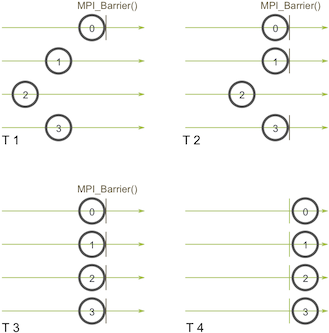
\includegraphics[width=0.7\linewidth]{day8_am/img/mpi/barrier.png}
                \caption{MPI\_Barrier}
                \label{fig:barrier}
            \end{figure}
        \end{column}
    \end{columns}
\end{frame}

\begin{frame}[fragile]{Broadcast: One to All}
    \begin{columns}
    
\begin{column}{.4\textwidth}
\begin{minted}[fontsize=\footnotesize]{c}
int MPI_Bcast(
    void* buffer,
    int count,
    MPI_Datatype datatype,
    int emitter_rank,
    MPI_Comm communicator);
\end{minted}

{\footnotesize
\begin{itemize}
    \item \textbf{emitter\_rank} 
The rank of the MPI process that broadcasts the data, all other processes receive the data broadcasted.
\end{itemize}
}
\end{column}

\begin{column}{.6\textwidth}
\begin{figure}
    \centering
    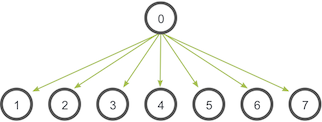
\includegraphics[width=0.75\linewidth]{day8_am/img/mpi/bcast.png}
    \caption{Bcast}
    \label{fig:bcast}
\end{figure}
\end{column}
\end{columns}
\end{frame}

\begin{frame}[fragile]{Broadcast: One to All}
\textbf{\large Why not Send and Receive?}

\begin{minted}[fontsize=\tiny]{c}
double start = MPI_Wtime();

if(my_rank == 0){
    for(int i=1; i<=31; i++)
        MPI_Send(sendbuf, 0x10000, MPI_INT, i, 0, MPI_COMM_WORLD);
}else{
    MPI_Recv(recvbuf, 0x10000, MPI_INT, 0, 0, MPI_COMM_WORLD, MPI_STATUS_IGNORE);
}

double end = MPI_Wtime();

if(my_rank == 0) printf("[Send Recv] Finished in %f seconds\n", my_rank, end-start);

start = MPI_Wtime();
MPI_Bcast(&sendbuf, 0x10000, MPI_INT, 0, MPI_COMM_WORLD);
end = MPI_Wtime();

if(my_rank == 0) printf("[Bcast] Finished in %f seconds\n", my_rank, end-start);
\end{minted}

\end{frame}

\begin{frame}{Broadcast: Tree based algorithm}
    \begin{figure}
        \centering
        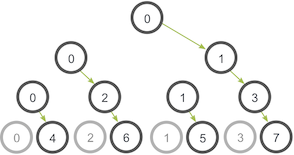
\includegraphics[width=0.65\linewidth]{day8_am/img/mpi/broadcasttree.png}
    \end{figure}
\end{frame}

\begin{frame}[fragile]{Scatter(One to All)}
    \begin{columns}
    
\begin{column}{.5\textwidth}
\begin{minted}[fontsize=\scriptsize]{c}
int MPI_Scatter(
    const void* buffer_send,
    int count_send,
    MPI_Datatype datatype_send,
    void* buffer_recv,
    int count_recv,
    MPI_Datatype datatype_recv,
    int root,
    MPI_Comm communicator);
\end{minted}

{\scriptsize
\begin{itemize}
    \item \textbf{count\_send}
    The number of elements to send to each process.

    \item \textbf{count\_receive}
    The number of elements in the receive buffer.
    
\end{itemize}
}
\end{column}

\begin{column}{.5\textwidth}
\begin{figure}
    \centering
    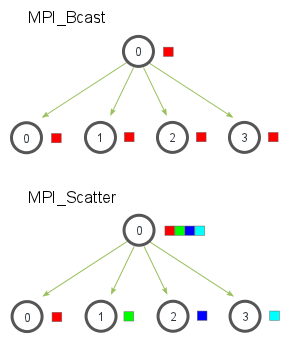
\includegraphics[width=0.8\linewidth]{day8_am/img/mpi/scatter.png}
    \caption{Scatter}
    \label{fig:scatter}
\end{figure}
\end{column}
\end{columns}
\end{frame}

\begin{frame}[fragile]{Gather: All to One}
    \begin{columns}
    
\begin{column}{.5\textwidth}
\begin{minted}[fontsize=\footnotesize]{c}
int MPI_Gather(
    const void* buffer_send,
    int count_send,
    MPI_Datatype datatype_send,
    void* buffer_recv,
    int count_recv,
    MPI_Datatype datatype_recv,
    int root,
    MPI_Comm communicator);
\end{minted}

\end{column}

\begin{column}{.5\textwidth}
\begin{figure}
    \centering
    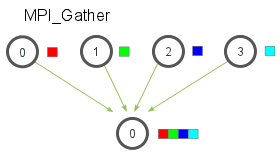
\includegraphics[width=0.75\linewidth]{day8_am/img/mpi/gather.png}
    \caption{MPI\_Gather}
\end{figure}
\end{column}
\end{columns}
\end{frame}

\begin{frame}[fragile]{Scatter and Gather}
    \begin{example}
        \textbf{Compute average}
    \end{example}
     \begin{minted}[fontsize=\scriptsize]{c}
MPI_Scatter(buffer, 0x1000000/4, MPI_DOUBLE, local_buffer, 0x1000000/4, MPI_DOUBLE, 0, MPI_COMM_WORLD);
double local_avg = 0;
for(int i=0; i<0x1000000/4; i++){
    local_avg += local_buffer[i];
}
local_avg /= 0x1000000/4;
double avgs[4];
MPI_Gather(&local_avg, 1, MPI_DOUBLE, avgs, 1, MPI_DOUBLE, 0, MPI_COMM_WORLD);
\end{minted}
\end{frame}

\begin{frame}[fragile]{Allgather(All to All)}
    \begin{columns}
    
\begin{column}{.5\textwidth}
\begin{minted}[fontsize=\footnotesize]{c}
int MPI_Allgather(
    const void* buffer_send,
    int count_send,
    MPI_Datatype datatype_send,
    void* buffer_recv,
    int count_recv,
    MPI_Datatype datatype_recv,
    MPI_Comm communicator);
\end{minted}

Actually MPI\_Gather + MPI\_Bcast.

\end{column}

\begin{column}{.5\textwidth}
\begin{figure}
    \centering
    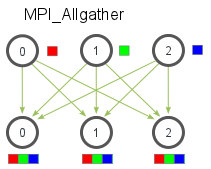
\includegraphics[width=0.75\linewidth]{day8_am/img/mpi/allgather.png}
    \caption{MPI\_Allgather}
    \label{fig:enter-label}
\end{figure}
\end{column}
\end{columns}
\end{frame}

\begin{frame}[fragile]{Reduce}
    \begin{columns}
    
\begin{column}{.5\textwidth}
\begin{minted}[fontsize=\footnotesize]{c}
int MPI_Reduce(
    const void* send_buffer,
    void* receive_buffer,
    int count,
    MPI_Datatype datatype,
    MPI_Op operation,
    int root,
    MPI_Comm communicator);
\end{minted}

\end{column}

\begin{column}{.5\textwidth}
\begin{figure}
    \centering
    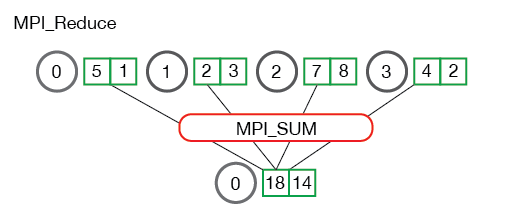
\includegraphics[width=0.75\linewidth]{day8_am/img/mpi/reduce.png}
    \caption{Reduce}
    \label{fig:reduce}
\end{figure}
\end{column}
\end{columns}
\end{frame}

\begin{frame}[fragile]{Reduce}
    \begin{example}
        \textbf{Compute average revisit}
    \end{example}
     \begin{minted}[fontsize=\scriptsize]{c}
MPI_Scatter(buffer, 0x1000000/4, MPI_DOUBLE, local_buffer, 0x1000000/4, MPI_DOUBLE, 0, MPI_COMM_WORLD);
double local_avg = 0;
for(int i=0; i<0x1000000/4; i++){
    local_avg += local_buffer[i];
}
local_avg /= 0x1000000/4;
double global_avg;
MPI_Reduce(&local_avg, &global_avg, 1, MPI_DOUBLE, MPI_SUM, 0, MPI_COMM_WORLD);
\end{minted}
\end{frame}